\section{Resultados}
\subsection{PCR em tempo real acomplado a High Resolution Melting Analysis}

A análise de HRM permite distinguir variantes de DNA com base em suas curvas de
dissociação térmica. As curvas de melting foram obtidas com o software High
Resolution Melt v.3.0.1 (Life Technologies), após a amplificação por PCR em
tempo real.

\begin{wrapfigure}{R}{.45\textwidth}
        \centering
        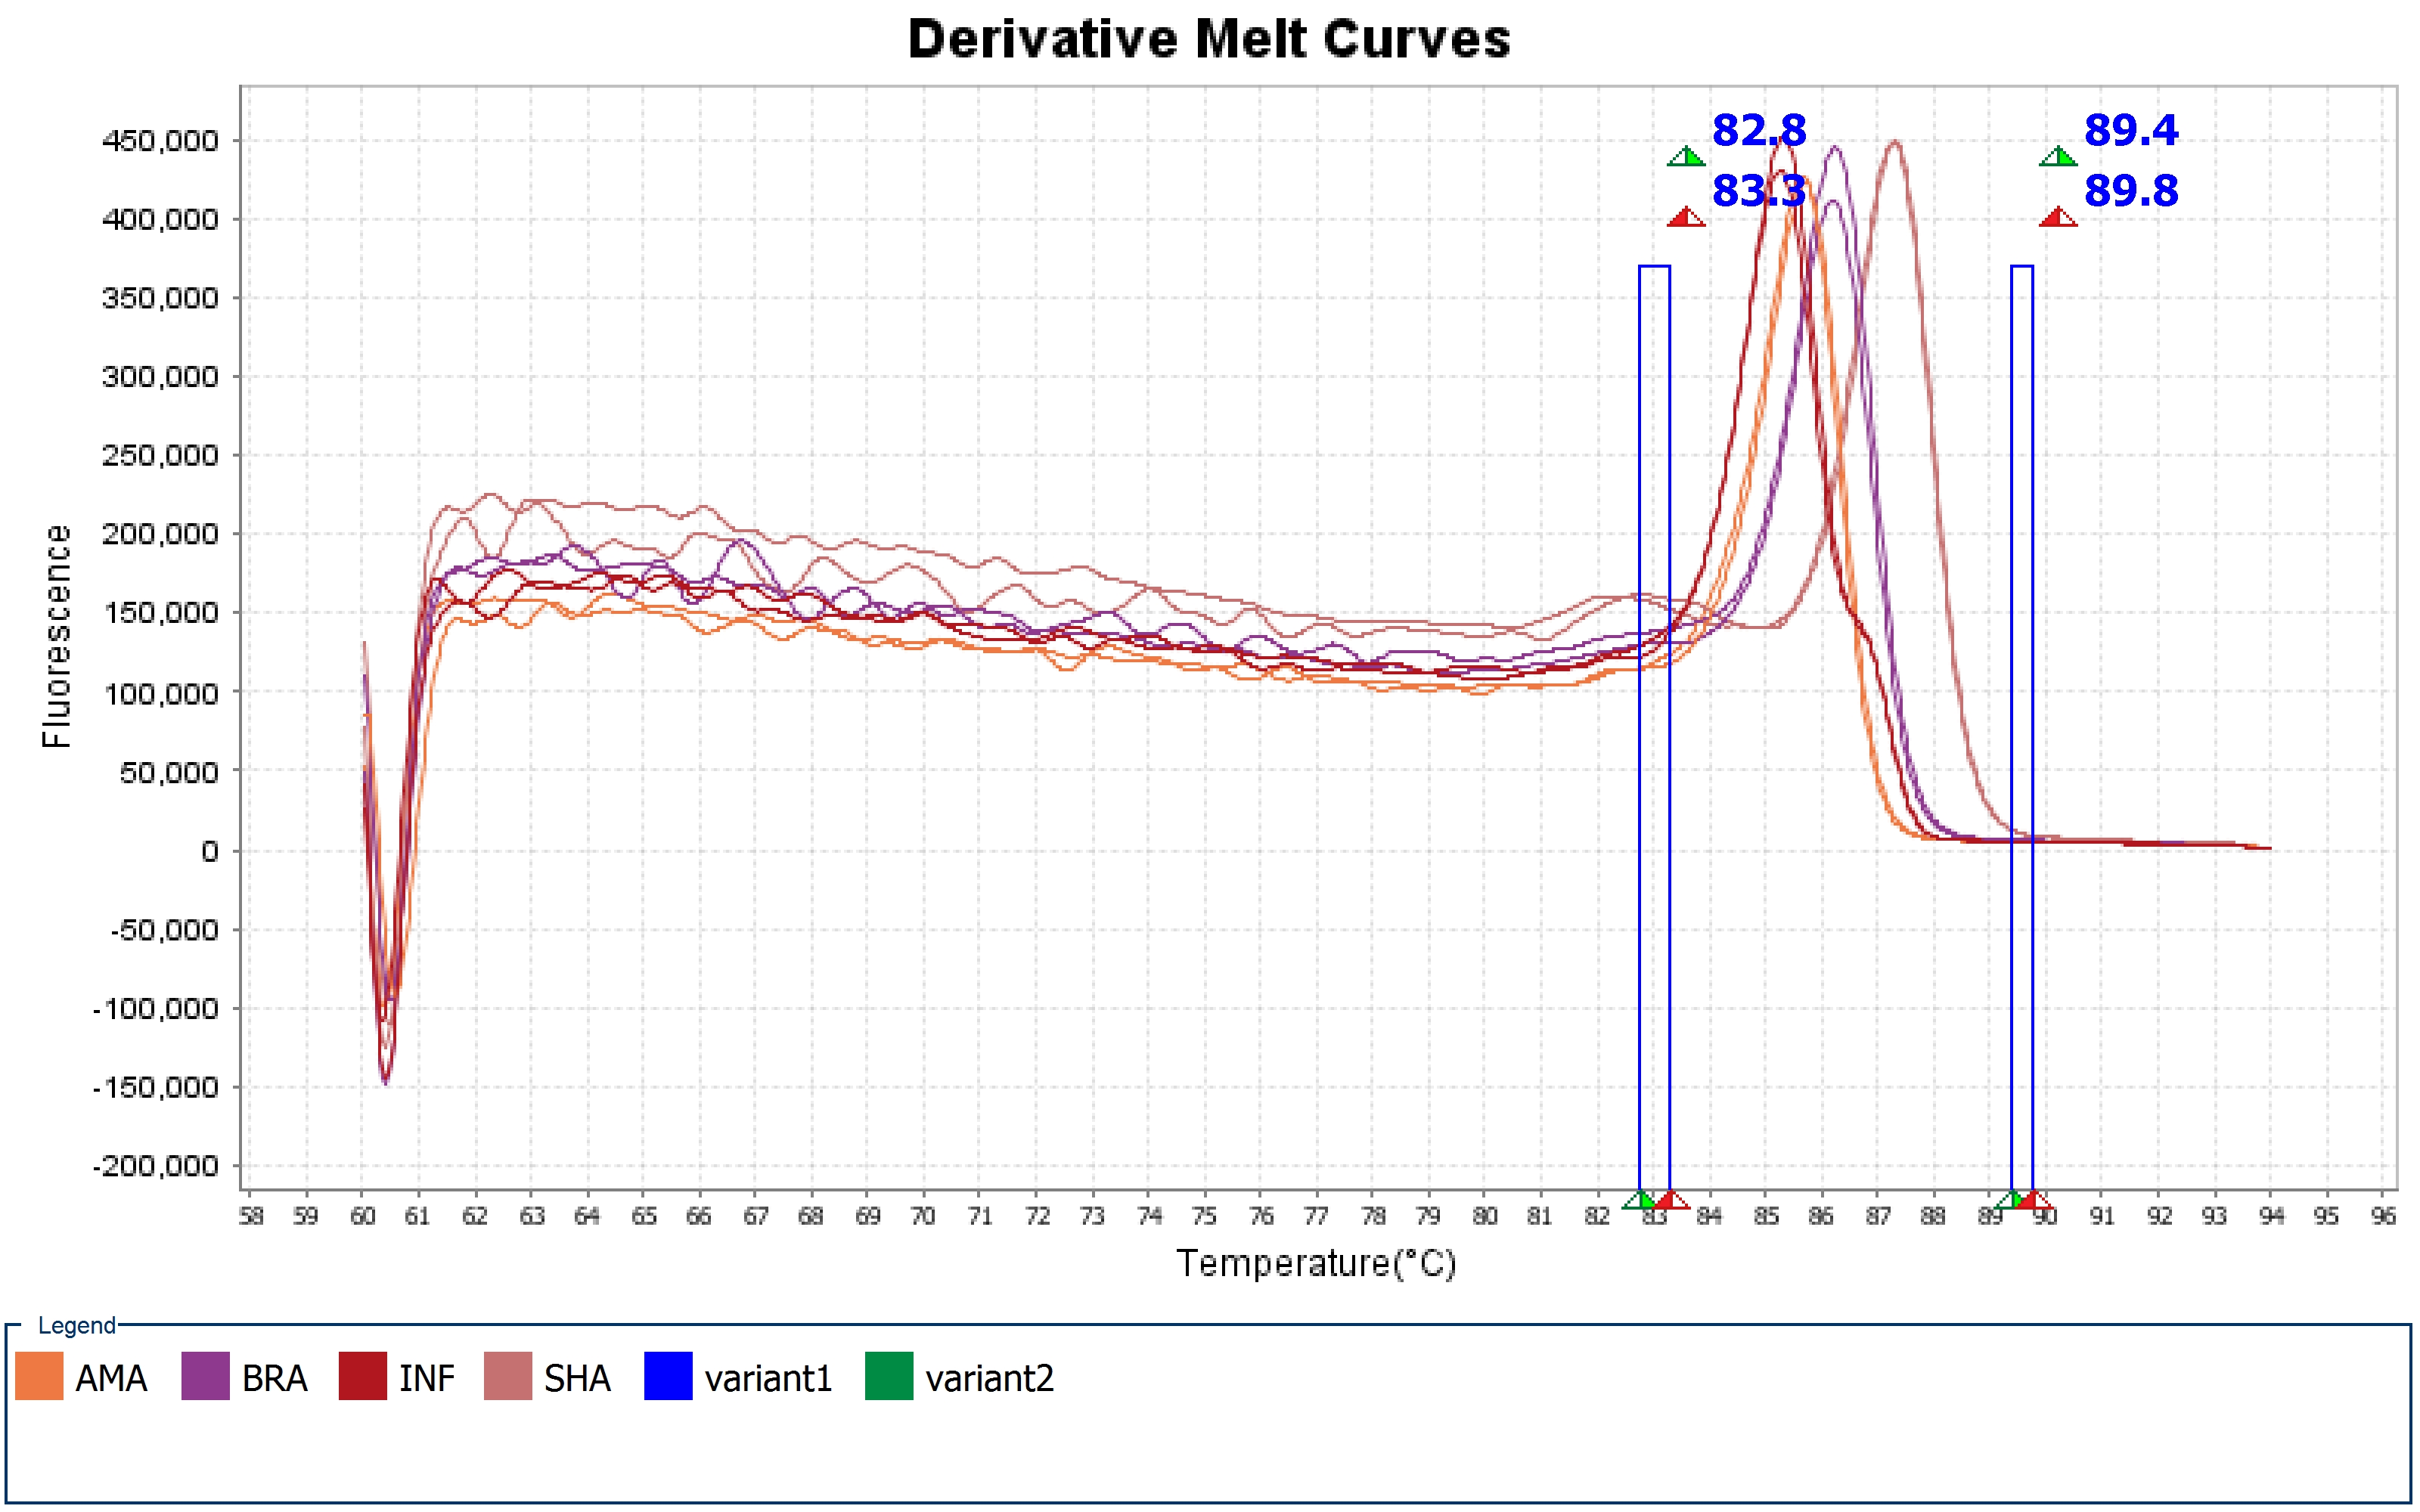
\includegraphics[width=.4\textwidth]{fig/Derivative Melt Curves.jpg}
        \caption{foto 1}
        \label{dmeltc}
        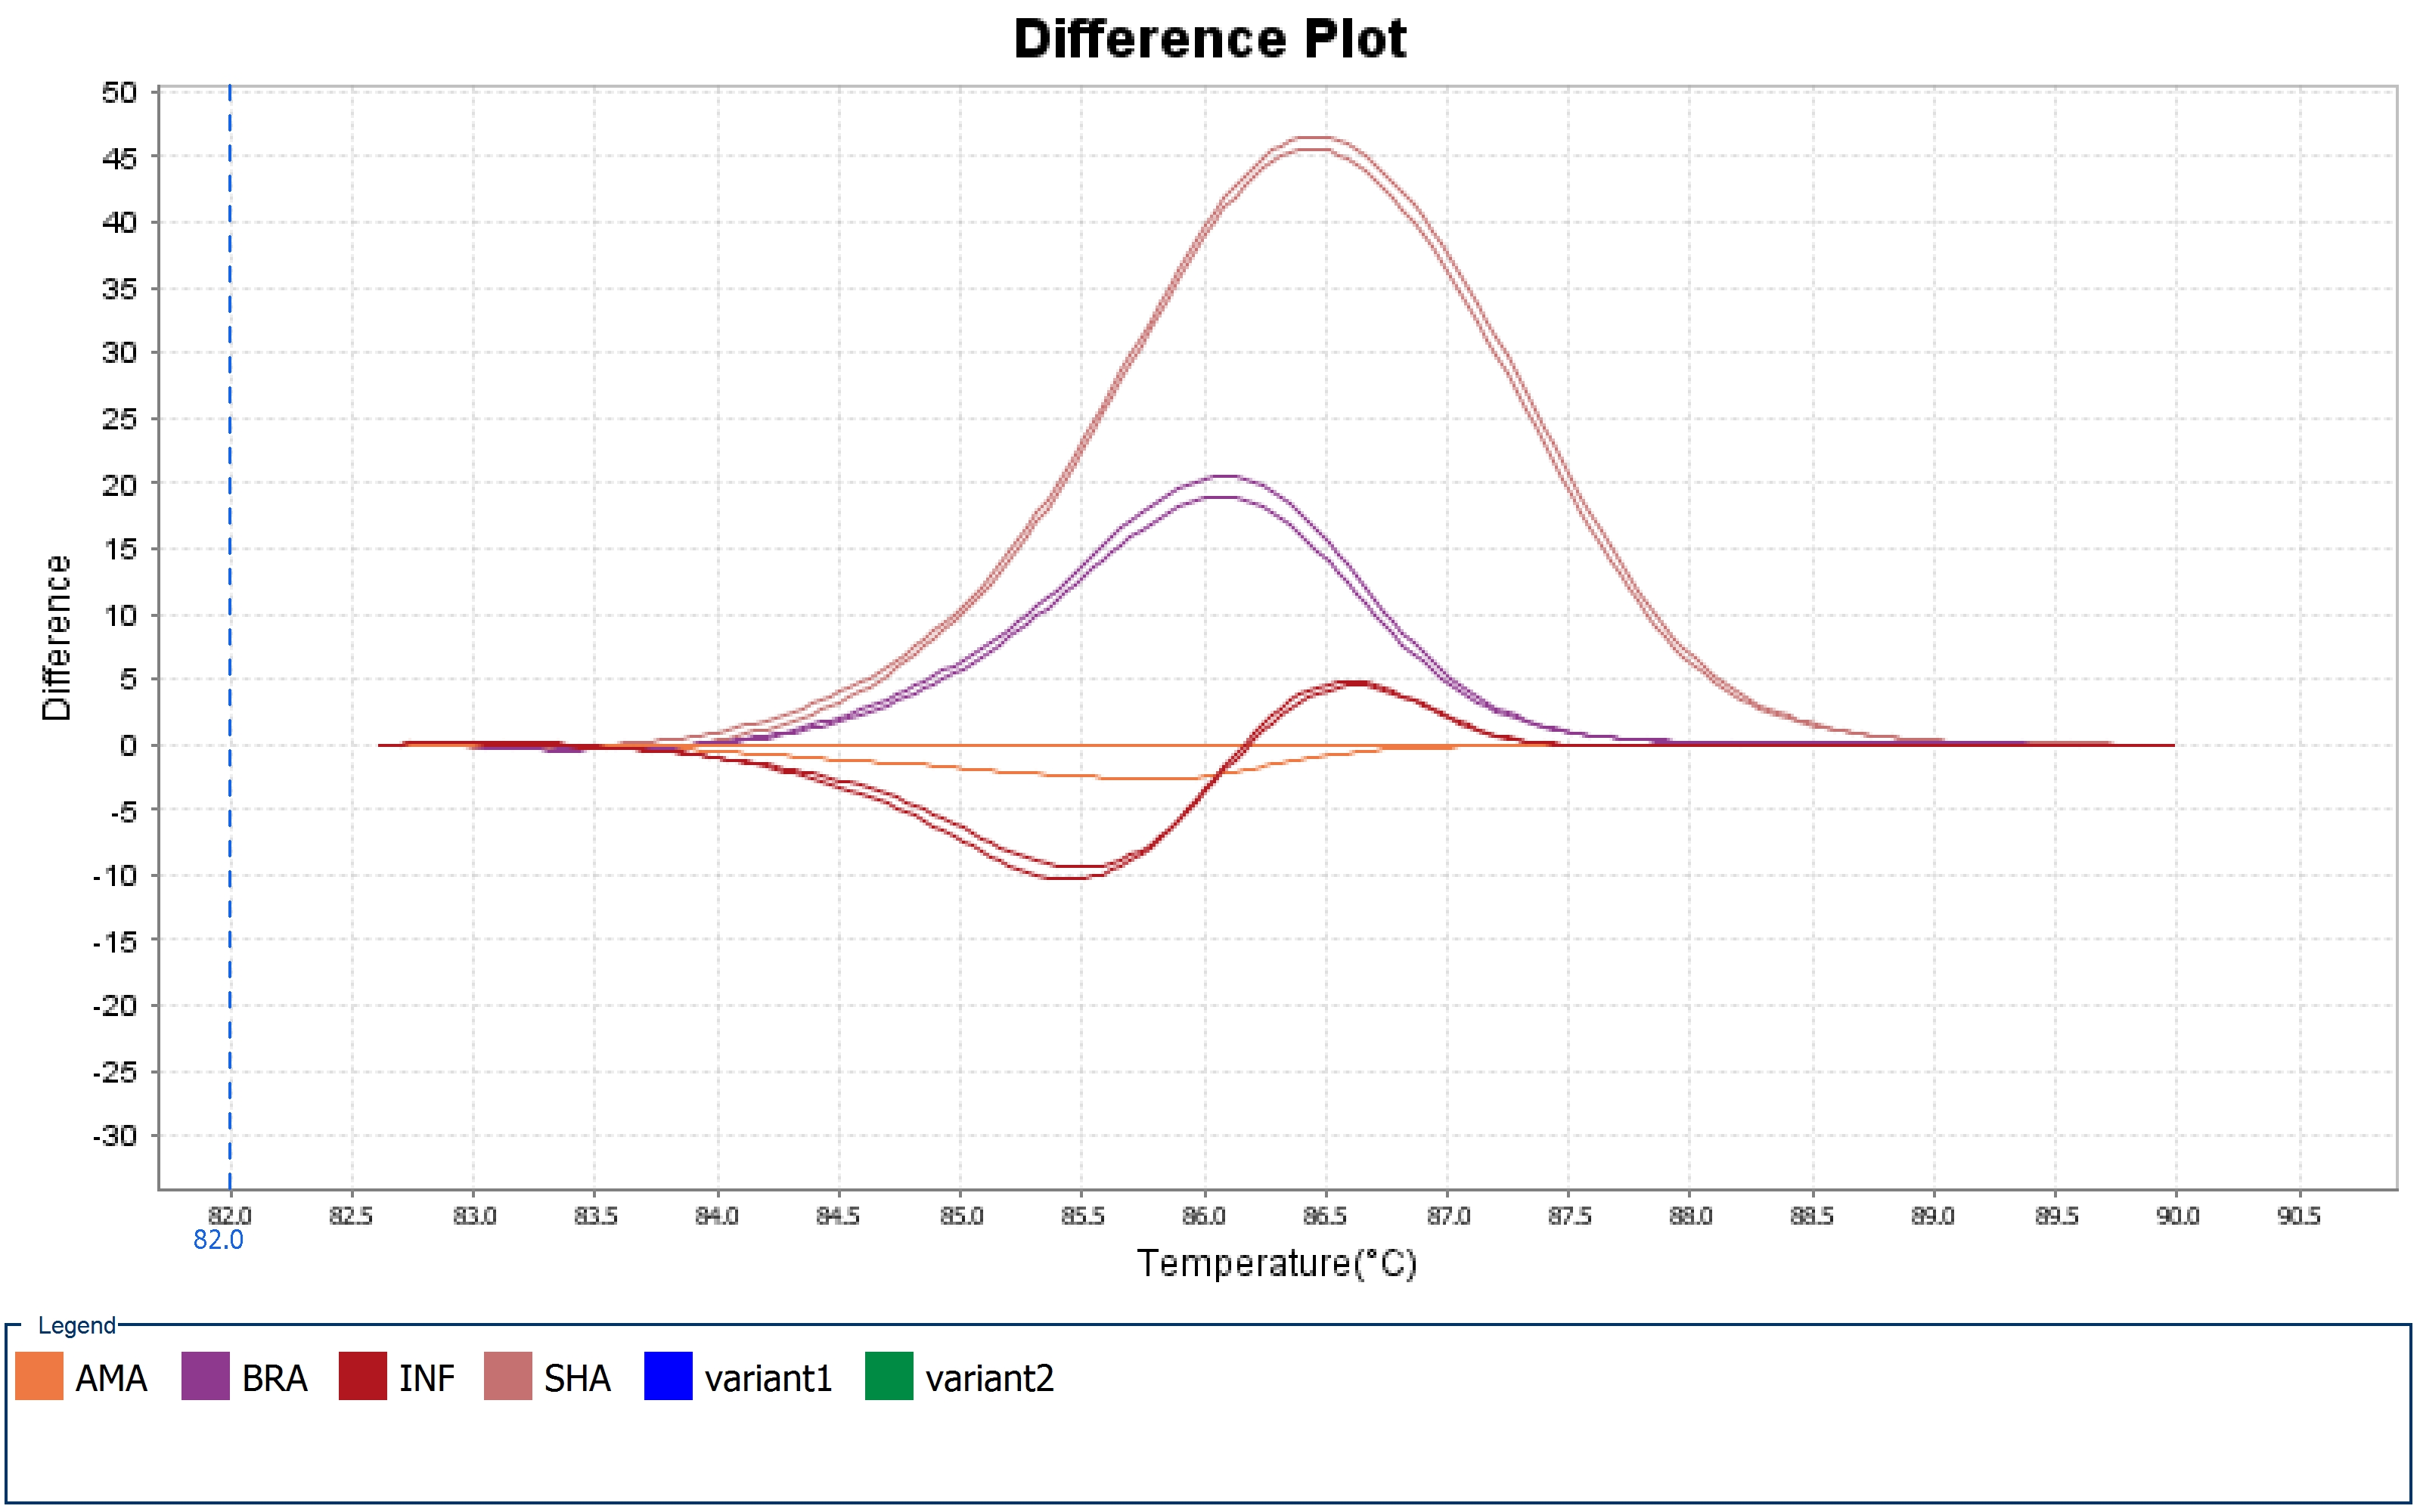
\includegraphics[width=.4\textwidth]{fig/Difference Plot.jpg}
        \caption{foto 1}
        \label{diffp}
        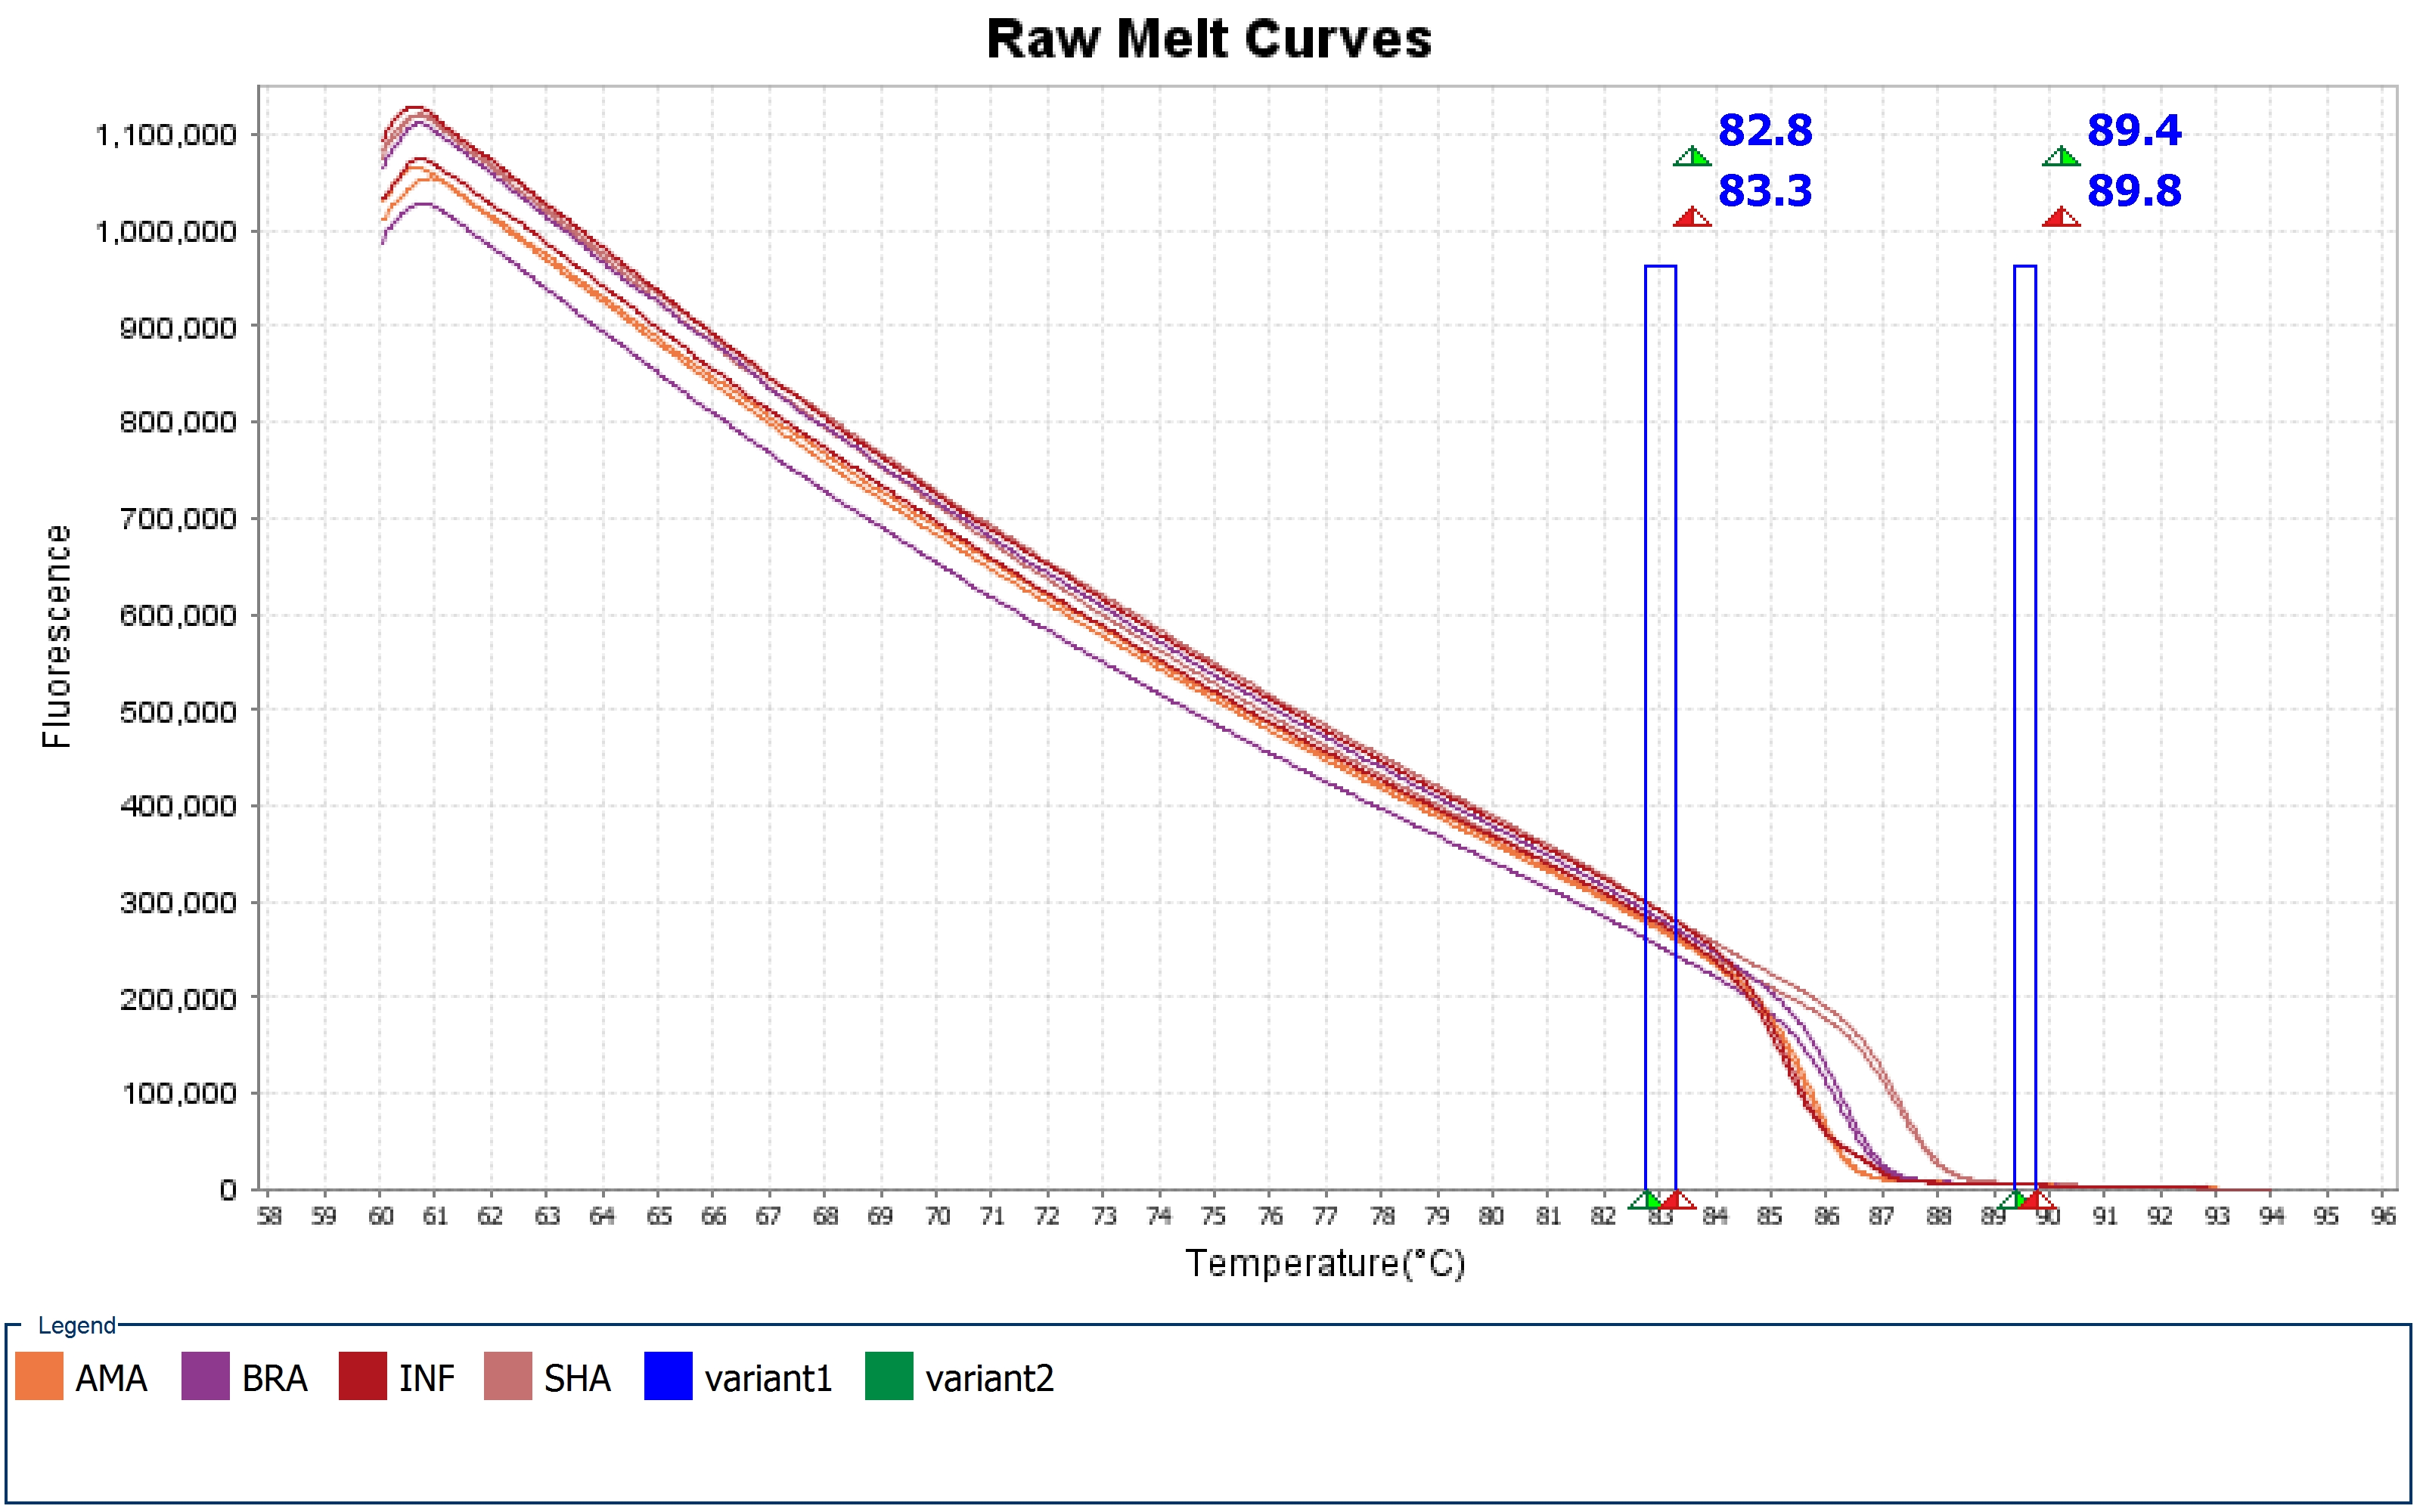
\includegraphics[width=.4\textwidth]{fig/Raw Melt Curves.jpg}
        \caption{Raw}
        \label{rawmelt}
\end{wrapfigure} %TODO: transformar imagens em uma prancheta, talvez não colocar
% como wrap fig... 

Primeiro, apenas com as amostras conhecidas, foram geradas as
\cref{dmeltc,diffp}. A
\cref{dmeltc} apresenta as curvas derivadas da fluorescência em função da
temperatura (derivative melt curves), nas quais os picos representam as
temperaturas de melting (Tm) específicas para cada amostra padronizada.

Para evidenciar as diferenças entre os perfis de melting das
amostras, foram geradas curvas de diferença (difference plots), apresentadas na
\cref{diffp}. 
É notável que cada espécie estudada
apresentou comportamento de melting único em comparação às demais. 

Por fim, a \cref{rawmelt} mostra as curvas normalizadas de reporter (normalised
reporter) em relação à
temperatura. Nesta é possível observar o padrão das amostras com \textit{L. (V.) shawi} e
\textit{L. (V.) brasilienses} que são visualmente distinguíveis. Já as curvas de
\textit{L. (L.) amazonensis} e \textit{L. (L.) infantum} são mais similares
entre si, embora facilmente distinguível das outras duas,  com
a maior diferença observável em valores pouco menores à \qty{87}{\celsius}.

\begin{wrapfigure}{L}{.45\textwidth}
        \centering
        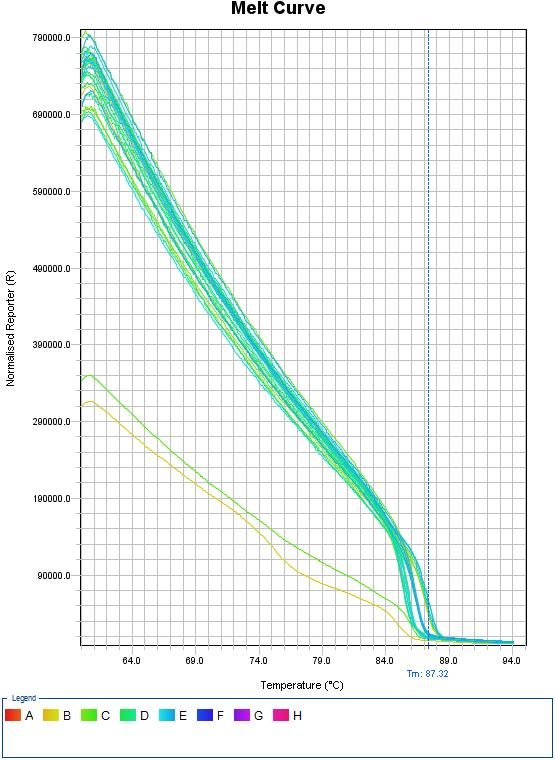
\includegraphics[width=.4\textwidth]{fig/Melt Curve.jpg}
        \caption{foto 1}
        \label{meltc}
        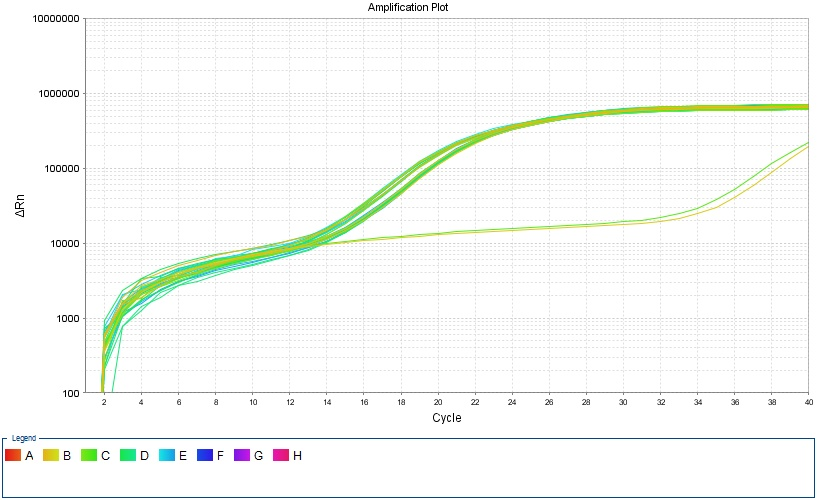
\includegraphics[width=.4\textwidth]{fig/Amplification Plot.jpg}
        \caption{foto 1}
        \label{amplip}
\end{wrapfigure}

As \cref{meltc,amplip} correspondem aos resultados da segunda reação de PCR em
tempo real, realizada com um conjunto de amostras desconhecidas acompanhadas de
controles positivos e negativos. A curva de melting apresentada na \cref{meltc}
revela que a maioria das amostras desconhecidas apresenta perfis de dissociação
compatíveis com os observados nas amostras padronizadas discutidas anteriormente
(\cref{dmeltc,diffp}), especialmente em relação aos valores de Tm, que podem ser
claramente identificados para cada amostra no gráfico.

Como esperado, duas curvas presentes na \cref{meltc} exibem perfis atípicos do
padrão observado nas curvas com as amostras conhecidas, estas duas curvas são
referentes aos dois poços com controle negativo. Isto é corroborado ao avaliar
as mesmas curvas na \cref{amplip}, que mostra as curvas de amplificação
correspondentes à mesma placa, em que esses dois poços não apresentaram aumento
significativo na fluorescência, comportamento compatível com o esperado para os
controles negativos incluídos na reação.

Ademais, na região de \qty{85}{\celsius}-\qty{88}{\celsius} da \cref{meltc} é
possível observar três padrões evidentemente diferentes e mais um que se
diferencia à pouco menos que \qty{87}{\celsius}. Estes são os mesmos quatro
padrões observados nas amostras conhecidas (\cref{rawmelt}).
